\documentclass{article}

\usepackage{amsmath}
\usepackage{float}
\usepackage{graphicx}
\usepackage{listings}
\usepackage{color}
\usepackage{hyperref}

\definecolor{dkgreen}{rgb}{0,0.6,0}
\definecolor{gray}{rgb}{0.5,0.5,0.5}
\definecolor{mauve}{rgb}{0.58,0,0.82}

\lstset{frame=tb,
    language=Python,
    aboveskip=3mm,
    belowskip=3mm,
    showstringspaces=false,
    columns=flexible,
    basicstyle={\small\ttfamily},
    numbers=none,
    numberstyle=\tiny\color{gray},
    keywordstyle=\color{blue},
    commentstyle=\color{dkgreen},
    stringstyle=\color{mauve},
    breaklines=true,
    breakatwhitespace=true,
    tabsize=3
}

\title{Assignment 3: Sentiment Analysis using Machine Learning}
\author{Aleksandr Jan Smoliakov}
\date{2024--12--10}

\begin{document}

\maketitle

\section{Introduction}

In this project, my objective is to build a machine learning model for sentiment analysis of tweets about US airlines. The dataset contains tweets along with their sentiment labels (positive, negative, or neutral). The goal is to classify the tweets into one of these three categories based on their text content.

The project will involve several steps, including analysis, dataset preprocessing, text cleaning, lemmatization, word cloud visualization, text vectorization, machine learning model training, and evaluation. I will use the Logistic Regression model for sentiment analysis due to its simplicity and interpretability.

\section{Methodology}

\subsection{Dataset}

The dataset used in this project is a subset of the \href{https://www.kaggle.com/crowdflower/twitter-airline-sentiment}{\textit{Twitter US Airline Sentiment}} dataset available on Kaggle. The dataset contains tweets about various US airlines, along with their sentiment labels (positive, negative, or neutral).

The dataset consists of 14,640 tweets, with 9,178 negative, 3,099 neutral, and 2,363 positive tweets, collected in February 2015. There are 15 columns in the dataset, including the tweet text, airline name, along with many irrelevant columns, such as the tweet ID, user ID, location, and more. For this project, I will only use two columns:

\begin{itemize}
    \item \texttt{text}: the tweet text, a short message between 12 and 186 characters.
    \item \texttt{airline\_sentiment}: the sentiment label (`positive', `negative', or `neutral').
\end{itemize}

\subsection{Dataset Preprocessing}

The first step in the pipeline is to preprocess the dataset to prepare it for the machine learning model. The following steps are performed:

\begin{itemize}
    \item \textbf{Removing Irrelevant Columns}: Remove all columns except for the \texttt{text} (the designated model inputs) and \texttt{airline\_sentiment} columns.
    \item \textbf{Checking for Missing Values}: Check for missing values in the dataset and remove any rows with missing text or sentiment labels.
    \item \textbf{Text Cleaning}: Perform text cleaning steps described below.
\end{itemize}

\subsubsection{Text Cleaning}

In order to prepare the text data for vectorization, I perform several preprocessing steps:

\begin{itemize}
    \item \textbf{Remove Twitter handles}: Completely remove Twitter handles (e.g., \texttt{@username}) that have high cardinality.
    \item \textbf{Remove URLs}: Completely remove URLs (e.g., \texttt{http://example.com}) that can produce a lot of distinct tokens.
    \item \textbf{Remove non-alphanumeric characters}: All characters except letters, numbers, and spaces are removed to keep the tokens clean.
    \item \textbf{Remove extra spaces}: Multiple spaces are replaced with a single space to facilitate tokenization.
    \item \textbf{Convert to lowercase}: Convert all text to lowercase to reduce the vocabulary size.
    \item \textbf{Tokenization}: Split the text into individual words (tokens) based on whitespace.
    \item \textbf{Remove stopwords}: Remove common words that do not carry much meaning (e.g., `the', `and', `is').
\end{itemize}

I create a new column \texttt{text\_cleaned} that contains the preprocessed text data. This column will be used for text vectorization.

\subsection{Lemmatization}

Lemmatization is the process of reducing words to their base or root form (e.g., `running' to `run', `better' to `good'). This helps to reduce the vocabulary size and improve the generalization of the model. I use the \texttt{nltk} library's WordNetLemmatizer to lemmatize the text data. The lemmatized text is stored in a new column \texttt{text\_cleaned\_lemmatized}.

I will compare the performance of the model with and without lemmatization to see if it improves the model's accuracy.

\subsection{Word Cloud Visualization}

A word cloud is a visual representation of text data, where the size of each word indicates its frequency in the dataset. This visualization will provide insights into the most frequent words associated with each sentiment category.

\subsection{Text Vectorization}

In order to feed the text data into a machine learning model, I need to convert the text into a numerical representation. This process is called text vectorization. In this project, I use the CountVectorizer from the \texttt{scikit-learn} library to convert the text data into a matrix of token counts.

Mathematically, this can be expressed as:

\[
\text{CountVectorizer}(\text{`I really really like this airline'}) = \begin{bmatrix}
0 & 0 & 0 & 1 & 2 & 1 & 1 & 1
\end{bmatrix}
\]

where each element in the vector represents the count of a specific word in the text. This way more frequent words will have higher values in the vector.

\subsection{Machine Learning Model}

For the sentiment analysis task, I use a machine learning model to classify the tweets into one of three categories: positive, negative, or neutral. I choose the Logistic Regression model for this task due to its simplicity, interpretability, and decent performance on text classification tasks.

The Python library \texttt{scikit-learn} provides an implementation of the Logistic Regression model that can be easily trained and evaluated. I randomly split the dataset into training (80\%) and testing (20\%) sets to train the model on the training set and evaluate its performance on the testing set.

\subsection{Evaluation Metrics}

Evaluation metrics are used to assess the performance of the machine learning model. For the sentiment analysis task, I use the following evaluation metrics:

\begin{itemize}
    \item \textbf{Accuracy}: The proportion of correctly classified tweets.
    \item \textbf{Precision}: The proportion of correctly classified positive tweets among all tweets classified as positive.
    \item \textbf{Recall}: The proportion of correctly classified positive tweets among all actual positive tweets.
    \item \textbf{F1 Score}: The harmonic mean of precision and recall, providing a balance between the two metrics.
\end{itemize}

\section{Analysis and Results}

In this section, I apply the methodology described above to the Twitter US Airline Sentiment dataset and analyze the results.

\subsection{Dataset Preprocessing and Lemmatization}

The dataset preprocessing steps are performed as described in the methodology section. Only two columns, \texttt{text} and \texttt{airline\_sentiment}, are retained for further analysis. There are no missing values in the dataset, thus no rows are removed. The text cleaning steps are applied to the \texttt{text} column, and the preprocessed text is stored in the \texttt{text\_cleaned} column. The lemmatization step is performed, and the lemmatized text is stored in the \texttt{text\_cleaned\_lemmatized} column.

\subsection{Word Cloud Visualization}

I created word cloud visualizations to explore the most common words in each sentiment category. The word clouds are presented in the Appendix 1.

Looking at the word clouds, it is clear that in every sentiment category, airline names (e.g., `united', `jetblue', `usairways') dominate the most frequent words. This is expected, as the dataset contains tweets about various US airlines.

I have decided against removing airline names from the text data, as they could be an important feature for sentiment analysis. The presence of airline names in the text can provide valuable information about the sentiment expressed towards a specific airline.

However, among them are also words that are more indicative of sentiment, such as `thanks', `great', `love', and `helpful' in the positive tweet wordcloud (Appendix 1, Figure~\ref{fig:positive_wordcloud}), and `cancelled', `delayed', `late', and `never' in the negative wordcloud (Appendix 1, Figure~\ref{fig:negative_wordcloud}).

The neutral wordcloud (Appendix 1, Figure~\ref{fig:neutral_wordcloud}) contains a salad of general airline-related words, such as `flight', `airport', airline names, and some (not many) words from both the polarized categories, such as `cancelled', `problems', but also `thank' and `good'. These words may have been used in a different context, or neutral tweets may contain a mix of positive and negative sentiments.

\subsection{Text Vectorization}

The preprocessed text data is converted into numerical features using the TF-IDF vectorizer with a maximum of 1,000 features. The features are generated from n-grams of words (1-grams and 2-grams) to capture both unigrams and bigrams in the text data. The resulting feature matrix has 14,640 rows (one for each tweet) and 1,000 columns (one for each unique word or word pair).

\subsection{Machine Learning Model}

Two Logistic Regression models are trained on the feature matrix, one with lemmatization and one without. The models are trained on 80\% of the dataset and evaluated on the remaining 20\%.

\subsection{Evaluation Metrics}

The accuracy metrics of the two models are presented in Table~\ref{tab:accuracy_metrics}. The fraction of the test set represented by the largest class (negative sentiment) is 0.645. Our best model, with lemmatization, achieves an accuracy of 0.793, which beats the baseline, but not by a large margin.

\begin{table}[H]
    \begin{tabular}{ccc}
        \hline
        \textbf{Metric} & \textbf{Without Lemmatization} & \textbf{With Lemmatization} \\
        \hline
        Accuracy & 0.788 & 0.793 \\
        \hline
    \end{tabular}
    \caption{\label{tab:accuracy_metrics} Accuracy metrics for the two models.}
\end{table}

Precision, recall, and F1 score metrics for each model and sentiment category are presented in Table~\ref{tab:precision_recall_f1}. The model performs well on the negative sentiment category, achieving high precision, recall, and F1 score. The neutral sentiment category has the lowest performance, with the model struggling to classify tweets correctly. The positive sentiment category has moderate performance, with precision and F1 score higher than recall.

\begin{table}[H]
    \begin{tabular}{cccc}
        \hline
        \textbf{Metric} & \textbf{Negative} & \textbf{Neutral} & \textbf{Positive} \\
        \hline
        Precision (without lemmatization) & 0.857 & 0.593 & 0.741 \\
        Recall (without lemmatization) & 0.873 & 0.591 & 0.686 \\
        F1 Score (without lemmatization) & 0.865 & 0.592 & 0.713 \\
        \hline
        Precision (with lemmatization) & 0.858 & 0.608 & 0.743 \\
        Recall (with lemmatization) & 0.881 & 0.591 & 0.686 \\
        F1 Score (with lemmatization) & 0.870 & 0.600 & 0.713 \\
        \hline
    \end{tabular}
    \caption{\label{tab:precision_recall_f1} Precision, recall, and F1 score metrics for each sentiment category.}
\end{table}

The confusion matrix for the (better) model with lemmatization is presented in Figure~\ref{fig:confusion_matrix_with_lemmatization}. The confusion matrix shows the number of true positive, true negative, false positive, and false negative predictions for each sentiment category.

\begin{figure}[H]
    \centering
    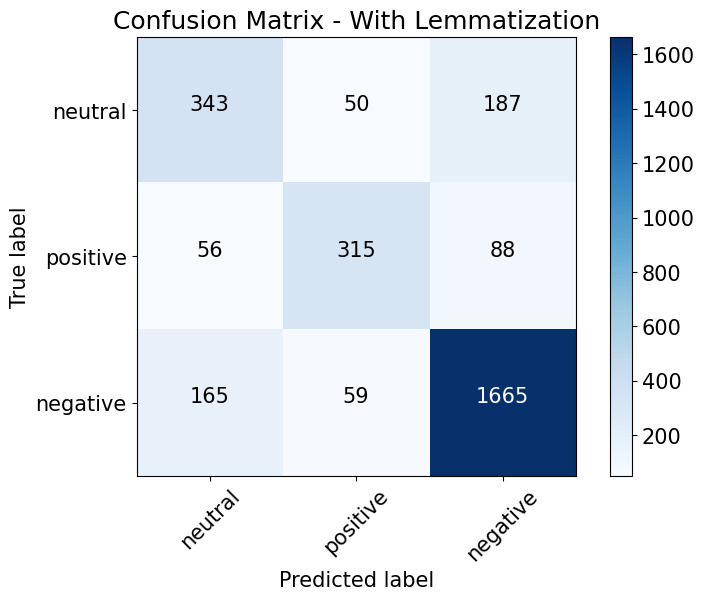
\includegraphics[width=0.8\textwidth]{data/plots/confusion_matrix_with_lemmatization.png}
    \caption{\label{fig:confusion_matrix_with_lemmatization} Confusion matrix for the model with lemmatization.}
\end{figure}

\section{Conclusions}

I have successfully built a machine learning model for sentiment analysis of tweets about US airlines. The model performs moderately well on the sentiment analysis task, achieving an accuracy of 0.793 with lemmatization and 0.788 without lemmatization.

The precision, recall, and F1 score are highest for the negative sentiment category and lowest for the neutral sentiment category. The fact that the model classifies negative tweets with high precision and recall reflects the dominance of negative tweets in the dataset. The neutral sentiment category is the most challenging to classify, as neutral tweets may contain a mix of positive and negative sentiments.

There is room for improvement in the model's performance, especially in classifying neutral tweets. Future work could involve experimenting with different balancing techniques, text vectorization techniques (e.g., word embeddings), machine learning models (e.g., neural networks), and hyperparameters to improve the model's performance. Additionally, exploring more advanced text preprocessing techniques and feature engineering could help improve the model's accuracy.

All in all, the model performs moderately well on the sentiment analysis task, but there is room for improvement. The insights gained from this project can be used to build more accurate sentiment analysis models for tweets about US airlines.

\section{Source Code}

The source code used in this solution is available in the Appendix 2.

\newpage

\section*{Appendix 1: Word Clouds}

\begin{figure}[!htbp]
    \centering
    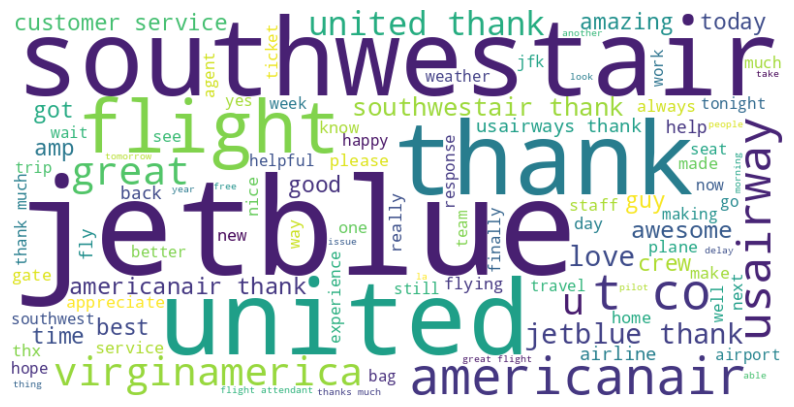
\includegraphics[width=\textwidth]{data/plots/positive_wordcloud.png}
    \caption{Word cloud visualization of positive tweets.}
    \label{fig:positive_wordcloud}
\end{figure}

\begin{figure}[!htbp]
    \centering
    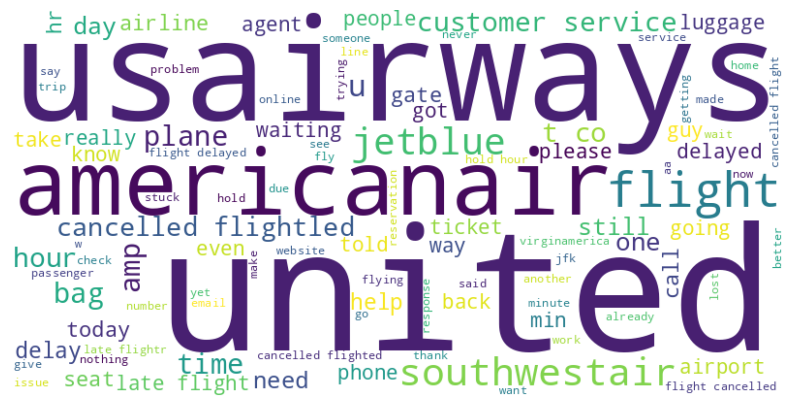
\includegraphics[width=\textwidth]{data/plots/negative_wordcloud.png}
    \caption{Word cloud visualization of negative tweets.}
    \label{fig:negative_wordcloud}
\end{figure}

\begin{figure}[!htbp]
    \centering
    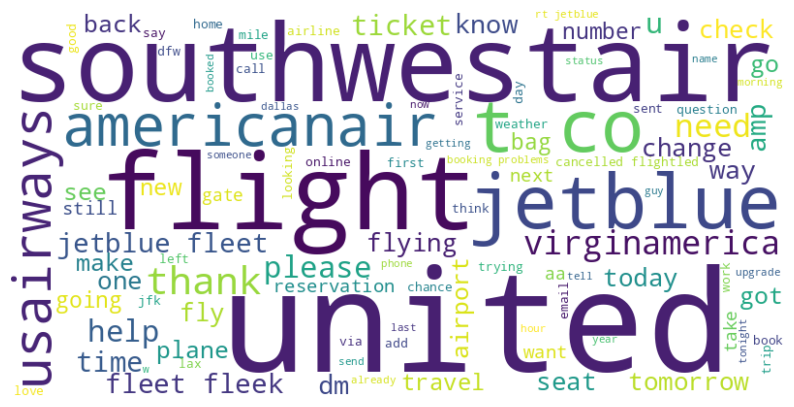
\includegraphics[width=\textwidth]{data/plots/neutral_wordcloud.png}
    \caption{Word cloud visualization of neutral tweets.}
    \label{fig:neutral_wordcloud}
\end{figure}

\newpage

\section*{Appendix 2: Source Code}

Source code used in this solution is presented below. The code is written in Python 3.11 and uses the following libraries: \texttt{pandas}, \texttt{matplotlib}, \texttt{nltk}, \texttt{scikit-learn}, \texttt{numpy}, and \texttt{wordcloud}.

\begin{lstlisting}
import itertools
import logging
import matplotlib.pyplot as plt
import numpy as np
import pandas as pd
from pathlib import Path
from wordcloud import WordCloud
from nltk.corpus import stopwords
from nltk.stem import WordNetLemmatizer
from sklearn.feature_extraction.text import CountVectorizer
from sklearn.linear_model import LogisticRegression
from sklearn.metrics import accuracy_score, classification_report, confusion_matrix
from sklearn.model_selection import train_test_split


logging.basicConfig(level=logging.INFO)

plt.rcParams.update({"font.size": 15})

# constants
INPUT_DIR = Path("data/input")
OUTPUT_DIR = Path("data/output")
PLOT_DIR = Path("data/plots")

STOP_WORDS = set(stopwords.words("english"))


def clean_text_column(column: pd.Series) -> pd.Series:
    # remove twitter handles
    column = column.str.replace(r"@[a-zA-Z0-9_]+", "")
    # remove URLs
    column = column.str.replace(r"http\S+", "")
    # remove special characters
    column = column.str.replace(r"[^a-zA-Z0-9\s]", "")
    # remove extra whitespaces
    column = column.str.replace(r"\s+", " ")
    # convert to lowercase
    column = column.str.lower()
    # tokenize the text
    column = column.str.strip().str.split()
    # remove stopwords
    column = column.apply(lambda x: [word for word in x if word not in STOP_WORDS])

    return column


def plot_word_clouds(df_data: pd.DataFrame, text_column: str) -> None:
    logging.info("Plotting word clouds...")

    # plot word clouds for each sentiment class
    for sentiment in df_data.airline_sentiment.unique():
        text = " ".join(
            df_data[df_data.airline_sentiment == sentiment][text_column].str.join(" ")
        )
        wordcloud = WordCloud(
            background_color="white",
            max_words=100,
            width=800,
            height=400,
            random_state=42,
        ).generate(text)

        plt.figure(figsize=(10, 6))
        plt.imshow(wordcloud, interpolation="bilinear")
        plt.axis("off")
        plt.savefig(PLOT_DIR / f"{sentiment}_wordcloud.png", bbox_inches="tight")
        logging.info(f"Word cloud for {sentiment} sentiment saved.")


def plot_confusion_matrix(
    y_true: pd.Series,
    y_pred: pd.Series,
    classes: list,
    title: str,
) -> None:
    cm = confusion_matrix(y_true, y_pred, labels=classes)

    plt.figure(figsize=(8, 6))
    plt.imshow(cm, interpolation="nearest", cmap=plt.cm.Blues)
    plt.title(title)
    plt.colorbar()
    tick_marks = np.arange(len(classes))
    plt.xticks(tick_marks, classes, rotation=45)
    plt.yticks(tick_marks, classes)

    thresh = cm.max() / 2.0
    for i, j in itertools.product(range(cm.shape[0]), range(cm.shape[1])):
        plt.text(
            j,
            i,
            format(cm[i, j], "d"),
            horizontalalignment="center",
            color="white" if cm[i, j] > thresh else "black",
        )

    filename = title.lower().replace("- ", "").replace(" ", "_")
    plt.tight_layout()
    plt.ylabel("True label")
    plt.xlabel("Predicted label")
    plt.savefig(PLOT_DIR / filename, bbox_inches="tight")
    logging.info(f"Confusion matrix saved as {filename}.png")


def fit_logistic_regression_model(
    df_data: pd.DataFrame,
    X_column: str,
    y_column: str,
    classes: list,
    title: str,
) -> None:
    X = df_data[X_column].str.join(" ")
    y = df_data[y_column]

    X_train, X_test, y_train, y_test = train_test_split(
        X, y, test_size=0.2, random_state=42
    )

    # applying tf-idf vectorization
    tfidf = CountVectorizer(
        max_features=2000,
        ngram_range=(1, 2),
    )
    X_train = tfidf.fit_transform(X_train)
    X_test = tfidf.transform(X_test)

    # split the data into training and testing sets
    logging.info(f"Training data shape: {X_train.shape}, {y_train.shape}")
    logging.info(f"Testing data shape: {X_test.shape}, {y_test.shape}")

    # train a classifier
    classifier = LogisticRegression(
        random_state=42,
        max_iter=1000,
    )
    classifier.fit(X_train, y_train)

    # evaluate the classifier
    y_pred = classifier.predict(X_test)
    accuracy = accuracy_score(y_test, y_pred)
    logging.info(f"Accuracy: {accuracy:.2f}")

    # per-class classification report
    logging.info(classification_report(y_test, y_pred, digits=3))

    # plot the confusion matrix
    plot_confusion_matrix(
        y_test,
        y_pred,
        classes=df_data.airline_sentiment.unique(),
        title=f"Confusion Matrix - {title}",
    )


def process_file(
    filename: Path,
) -> None:
    # load the csv file
    df_data = pd.read_csv(filename, parse_dates=True)
    logging.info(f"Data shape: {df_data.shape}")
    logging.info(f"Columns: {df_data.columns}")

    logging.info(f"Class distribution:")
    logging.info(df_data.airline_sentiment.value_counts())

    logging.info(f"Tweet length statistics:")
    logging.info(df_data.text.str.len().describe())

    # removing irrelevant columns
    df_data = df_data[["airline_sentiment", "text"]]

    # removing rows with missing values
    logging.info(f"Rows with missing values:")
    logging.info(f"{df_data.isnull().sum(axis=0)}")
    df_data = df_data.dropna()

    # cleaning text data
    df_data["text_cleaned"] = clean_text_column(df_data["text"])

    # plotting the word clouds
    # plot_word_clouds(df_data, text_column="text_cleaned")

    # lemmatizing the text data
    lemmatizer = WordNetLemmatizer()
    df_data["text_cleaned_lemmatized"] = df_data["text_cleaned"].apply(
        lambda x: [lemmatizer.lemmatize(word) for word in x]
    )

    # fitting a logistic regression model without lemmatization
    logging.info("Fitting a logistic regression model without lemmatization...")
    fit_logistic_regression_model(
        df_data,
        X_column="text_cleaned",
        y_column="airline_sentiment",
        classes=df_data.airline_sentiment.unique(),
        title="Without Lemmatization",
    )

    # fitting a logistic regression model with lemmatization
    logging.info("Fitting a logistic regression model with lemmatization...")
    fit_logistic_regression_model(
        df_data,
        X_column="text_cleaned_lemmatized",
        y_column="airline_sentiment",
        classes=df_data.airline_sentiment.unique(),
        title="With Lemmatization",
    )


if __name__ == "__main__":
    # create directories if they don't exist
    INPUT_DIR.mkdir(parents=True, exist_ok=True)
    OUTPUT_DIR.mkdir(parents=True, exist_ok=True)
    PLOT_DIR.mkdir(parents=True, exist_ok=True)

    filenames = list(INPUT_DIR.glob("*.csv"))

    # validate input files
    assert len(filenames) > 0, "No input files provided."

    # process each csv file
    for filename in filenames:
        logging.info(f"Processing {filename}")
        process_file(
            filename,
        )
        logging.info("\n")
\end{lstlisting}

\end{document}
